\begin{equation}
    \begin{gathered}
        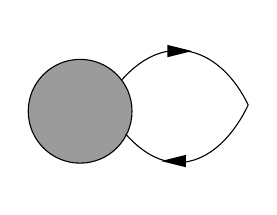
\begin{tikzpicture}[x=0.75pt,y=0.75pt,yscale=-1,xscale=1]
            %uncomment if require: \path (0,300); %set diagram left start at 0, and has height of 300
            
            %Shape: Circle [id:dp9547132007370212] 
            \draw  [fill={rgb, 255:red, 155; green, 155; blue, 155 }  ,fill opacity=1 ] (56,136) .. controls (56,122.19) and (67.19,111) .. (81,111) .. controls (94.81,111) and (106,122.19) .. (106,136) .. controls (106,149.81) and (94.81,161) .. (81,161) .. controls (67.19,161) and (56,149.81) .. (56,136) -- cycle ;
            %Curve Lines [id:da4224241216982587] 
            \draw    (101,121) .. controls (123,96) and (149,106) .. (162,133) ;
            %Curve Lines [id:da07143179889536055] 
            \draw    (103,147) .. controls (125,172) and (149,160) .. (162,133) ;
            %Straight Lines [id:da4398750229808517] 
            \draw    (135,107) ;
            \draw [shift={(135,107)}, rotate = 180] [fill={rgb, 255:red, 0; green, 0; blue, 0 }  ][line width=0.08]  [draw opacity=0] (12,-3) -- (0,0) -- (12,3) -- cycle    ;
            %Straight Lines [id:da25703305779579977] 
            \draw    (129,160) -- (122,160) ;
            \draw [shift={(120,160)}, rotate = 360] [fill={rgb, 255:red, 0; green, 0; blue, 0 }  ][line width=0.08]  [draw opacity=0] (12,-3) -- (0,0) -- (12,3) -- cycle    ;
            \end{tikzpicture}            
    \end{gathered} \quad = \quad  \begin{gathered}
        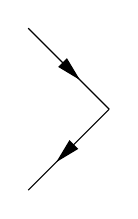
\begin{tikzpicture}[x=0.75pt,y=0.75pt,yscale=-1,xscale=1]
            %uncomment if require: \path (0,300); %set diagram left start at 0, and has height of 300
            
            %Straight Lines [id:da5267990075099112] 
            \draw    (100,121) -- (139,160) ;
            %Straight Lines [id:da17272928206943328] 
            \draw    (139,160) -- (100,199) ;
            %Straight Lines [id:da957803192854821] 
            \draw    (119.5,140.5) -- (123.59,144.59) ;
            \draw [shift={(125,146)}, rotate = 225] [fill={rgb, 255:red, 0; green, 0; blue, 0 }  ][line width=0.08]  [draw opacity=0] (12,-3) -- (0,0) -- (12,3) -- cycle    ;
            %Straight Lines [id:da3141174634629429] 
            \draw    (119.5,179.5) -- (114.91,184.09) ;
            \draw [shift={(113.5,185.5)}, rotate = 315] [fill={rgb, 255:red, 0; green, 0; blue, 0 }  ][line width=0.08]  [draw opacity=0] (12,-3) -- (0,0) -- (12,3) -- cycle    ;
            \end{tikzpicture}            
    \end{gathered} \quad + \quad \begin{gathered}
        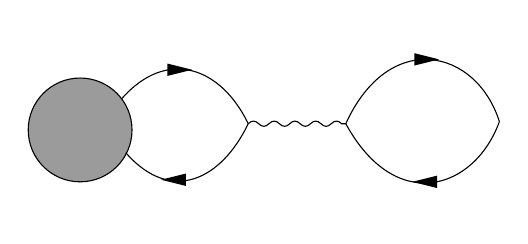
\begin{tikzpicture}[x=0.75pt,y=0.75pt,yscale=-1,xscale=1]
            %uncomment if require: \path (0,300); %set diagram left start at 0, and has height of 300
            
            %Shape: Circle [id:dp9547132007370212] 
            \draw  [fill={rgb, 255:red, 155; green, 155; blue, 155 }  ,fill opacity=1 ] (56,136) .. controls (56,122.19) and (67.19,111) .. (81,111) .. controls (94.81,111) and (106,122.19) .. (106,136) .. controls (106,149.81) and (94.81,161) .. (81,161) .. controls (67.19,161) and (56,149.81) .. (56,136) -- cycle ;
            %Curve Lines [id:da4224241216982587] 
            \draw    (101,121) .. controls (123,96) and (149,106) .. (162,133) ;
            %Curve Lines [id:da07143179889536055] 
            \draw    (103,147) .. controls (125,172) and (149,160) .. (162,133) ;
            %Straight Lines [id:da4398750229808517] 
            \draw    (135,107) ;
            \draw [shift={(135,107)}, rotate = 180] [fill={rgb, 255:red, 0; green, 0; blue, 0 }  ][line width=0.08]  [draw opacity=0] (12,-3) -- (0,0) -- (12,3) -- cycle    ;
            %Straight Lines [id:da25703305779579977] 
            \draw    (129,160) -- (122,160) ;
            \draw [shift={(120,160)}, rotate = 360] [fill={rgb, 255:red, 0; green, 0; blue, 0 }  ][line width=0.08]  [draw opacity=0] (12,-3) -- (0,0) -- (12,3) -- cycle    ;
            %Curve Lines [id:da7048949301311622] 
            \draw    (209,133) .. controls (230,87) and (272,97) .. (283,132) ;
            %Curve Lines [id:da9048001439980424] 
            \draw    (209,133) .. controls (233,177) and (271,165) .. (283,132) ;
            %Straight Lines [id:da32267260611388426] 
            \draw    (254,102) ;
            \draw [shift={(254,102)}, rotate = 180] [fill={rgb, 255:red, 0; green, 0; blue, 0 }  ][line width=0.08]  [draw opacity=0] (12,-3) -- (0,0) -- (12,3) -- cycle    ;
            %Straight Lines [id:da310042974722734] 
            \draw    (250,161) -- (243,161) ;
            \draw [shift={(241,161)}, rotate = 360] [fill={rgb, 255:red, 0; green, 0; blue, 0 }  ][line width=0.08]  [draw opacity=0] (12,-3) -- (0,0) -- (12,3) -- cycle    ;
            %Straight Lines [id:da6796744681944953] 
            \draw    (162,133) .. controls (163.67,131.33) and (165.33,131.33) .. (167,133) .. controls (168.67,134.67) and (170.33,134.67) .. (172,133) .. controls (173.67,131.33) and (175.33,131.33) .. (177,133) .. controls (178.67,134.67) and (180.33,134.67) .. (182,133) .. controls (183.67,131.33) and (185.33,131.33) .. (187,133) .. controls (188.67,134.67) and (190.33,134.67) .. (192,133) .. controls (193.67,131.33) and (195.33,131.33) .. (197,133) .. controls (198.67,134.67) and (200.33,134.67) .. (202,133) .. controls (203.67,131.33) and (205.33,131.33) .. (207,133) -- (209,133) -- (209,133) ;
            \end{tikzpicture}            
    \end{gathered},
\end{equation}